\documentclass[12pt]{article}
\usepackage{times} 			% use Times New Roman font

\usepackage[margin=1in]{geometry}   % sets 1 inch margins on all sides
\usepackage[hidelinks]{hyperref}               % for URL formatting
\usepackage[pdftex]{graphicx}       % So includegraphics will work
\setlength{\parskip}{1em}           % skip 1em between paragraphs
\usepackage{indentfirst}            % indent the first line of each paragraph
\usepackage{datetime}
\usepackage[small, bf]{caption}
\usepackage{listings}               % for code listings
\usepackage{xcolor}                 % for styling code
\usepackage{multirow}
\usepackage{subcaption}     % for subfigures

%\setlength\intextsep{1.69cm} 

%New colors defined below
\definecolor{backcolour}{RGB}{246, 246, 246}   % 0xF6, 0xF6, 0xF6
\definecolor{codegreen}{RGB}{16, 124, 2}       % 0x10, 0x7C, 0x02
\definecolor{codepurple}{RGB}{170, 0, 217}     % 0xAA, 0x00, 0xD9
\definecolor{codered}{RGB}{154, 0, 18}         % 0x9A, 0x00, 0x12

%Code listing style named "gcolabstyle" - matches Google Colab
\lstdefinestyle{gcolabstyle}{
  basicstyle=\ttfamily\small,
  backgroundcolor=\color{backcolour},   
  commentstyle=\itshape\color{codegreen},
  keywordstyle=\color{codepurple},
  stringstyle=\color{codered},
  numberstyle=\ttfamily\footnotesize\color{darkgray}, 
  breakatwhitespace=false,         
  breaklines=true,                 
  captionpos=b,                    
  keepspaces=true,                 
  numbers=left,                    
  numbersep=5pt,                  
  showspaces=false,                
  showstringspaces=false,
  showtabs=false,                  
  tabsize=2
}

\lstset{style=gcolabstyle}      %set gcolabstyle code listing

% to make long URIs break nicely
\makeatletter
\g@addto@macro{\UrlBreaks}{\UrlOrds}
\makeatother

% for fancy page headings
\usepackage{fancyhdr}
\setlength{\headheight}{13.6pt} % to remove fancyhdr warning
\pagestyle{fancy}
\fancyhf{}
\rhead{\small \thepage}
\chead{\small CS 432, Spring 2024} 
\lhead{\small EC 0.6, Wilkinson}  % EDIT THIS, REPLACE # with HW number

%-------------------------------------------------------------------------
\begin{document}

% EDIT THE ITEMS HERE
\begin{centering}
{\large\textbf{EC 0.6 - Reports}}\\ 
Ryan Wilkinson\\
1/21/23\\
\end{centering}

%-------------------------------------------------------------------------

Figure \ref{fig:web-growth} shows a picture of delicious oranges freshly harvested this morning.

\begin{figure}[h!]
    \centering
    % trim and clip are used to crop the image, trim=left bottom right top
    % width sets max width, height will be scaled appropriately
    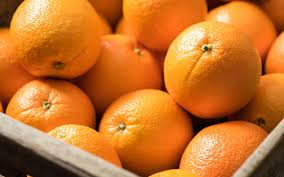
\includegraphics[trim=0 20 10 50, clip, width=\textwidth] {oranges.jpg}
    \caption{A photo of some delicious oranges!}
    \label{fig:web-growth}
\end{figure}

Listing \ref{lst:copy} is example code that was extracted from my submission of EC 0.1:

%Python code highlighting
\begin{lstlisting}[language=Python, caption=Python code extracted from EC 0.1, label=lst:copy]
#!/usr/local/bin/python3
# testargs.py

import sys

# Name: Ryan Wilkinson
# Resources used: https://www.w3schools.com/python/pandas/pandas_csv.asp

import pandas as pd

friend_count_data = pd.read_csv('friend-count.csv')
summary_data = [0] * 26
name_count = [0] * 26

for index, row in friend_count_data.iterrows():
    # Designate columns
    user = row[0]
    friend_count = row[1]

    # Convert the first letter of each user to an ASCII integer
    first_letter = ord(user[0])
    # If first_letter is >= a
    if first_letter >= 97:
        first_letter -= 97
    # if first_letter is >= A
    elif first_letter >= 65:
        first_letter -= 65

    # Assign the calculated first_letter to the 26-character summary_data table and
    # add the friend count
    summary_data[first_letter] = summary_data[first_letter] + friend_count
    name_count[first_letter] += 1

# Print the results
for index, total_friends in enumerate(summary_data):
    letter = index + 65
    print(chr(letter), "-", name_count[index], "users,", total_friends, "total friends")
\end{lstlisting}

Table \ref{tbl:simple} shows a table that outlines the class schedule for the first four weeks of CS 432.

\begin{table}[h]
\centering
\caption{CS 432 Schedule (first four weeks)}
\label{tbl:simple}
\begin{tabular}{|l|l|l|}
\hline
\textbf{Week} & \textbf{Date} & \textbf{Topic} \\ \hline \hline
1 & Jan 6 & Introduction to Web Science and Web Architecture \\ \hline
2 & Jan 13 & Introduction to Python \\ \hline
3 & Jan 20 & Measuring the Web \\ \hline
4 & Jan 27 & Searching the Web \\ \hline
\end{tabular}
\end{table}

\section*{References}

\begin{itemize}
    \item {Web Science: An Interdisciplinary Approach to Understanding the Web, \url{https://cacm.acm.org/magazines/2008/7/5366-web-science/fulltext}}
    \item{We knew the web was big...,
    \url{https://googleblog.blogspot.com/2008/07/we-knew-web-was-big.html}}
    \item{The Structure of the Web,
    \url{https://www.cs.cornell.edu/home/kleinber/networks-book/networks-book-ch13.pdf}}
\end{itemize}

\end{document}